% (find-LATEX "2023-1-C2-fracoes-parciais.tex")
% (defun c () (interactive) (find-LATEXsh "lualatex -record 2023-1-C2-fracoes-parciais.tex" :end))
% (defun C () (interactive) (find-LATEXsh "lualatex 2023-1-C2-fracoes-parciais.tex" "Success!!!"))
% (defun D () (interactive) (find-pdf-page      "~/LATEX/2023-1-C2-fracoes-parciais.pdf"))
% (defun d () (interactive) (find-pdftools-page "~/LATEX/2023-1-C2-fracoes-parciais.pdf"))
% (defun e () (interactive) (find-LATEX "2023-1-C2-fracoes-parciais.tex"))
% (defun o () (interactive) (find-LATEX "2022-2-C2-fracoes-parciais.tex"))
% (defun u () (interactive) (find-latex-upload-links "2023-1-C2-fracoes-parciais"))
% (defun v () (interactive) (find-2a '(e) '(d)))
% (defun d0 () (interactive) (find-ebuffer "2023-1-C2-fracoes-parciais.pdf"))
% (defun cv () (interactive) (C) (ee-kill-this-buffer) (v) (g))
%          (code-eec-LATEX "2023-1-C2-fracoes-parciais")
% (find-pdf-page   "~/LATEX/2023-1-C2-fracoes-parciais.pdf")
% (find-sh0 "cp -v  ~/LATEX/2023-1-C2-fracoes-parciais.pdf /tmp/")
% (find-sh0 "cp -v  ~/LATEX/2023-1-C2-fracoes-parciais.pdf /tmp/pen/")
%     (find-xournalpp "/tmp/2023-1-C2-fracoes-parciais.pdf")
%   file:///home/edrx/LATEX/2023-1-C2-fracoes-parciais.pdf
%               file:///tmp/2023-1-C2-fracoes-parciais.pdf
%           file:///tmp/pen/2023-1-C2-fracoes-parciais.pdf
%  http://anggtwu.net/LATEX/2023-1-C2-fracoes-parciais.pdf
% (find-LATEX "2019.mk")
% (find-sh0 "cd ~/LUA/; cp -v Pict2e1.lua Pict2e1-1.lua Piecewise1.lua ~/LATEX/")
% (find-sh0 "cd ~/LUA/; cp -v Pict2e1.lua Pict2e1-1.lua Pict3D1.lua ~/LATEX/")
% (find-sh0 "cd ~/LUA/; cp -v C2Subst1.lua C2Formulas1.lua ~/LATEX/")
% (find-sh0 "cd ~/LUA/; cp -v Gram2.lua Tree1.lua Caepro5.lua ~/LATEX/")
% (find-Deps1-links "Caepro5 Piecewise1")
% (find-Deps1-cps   "Caepro5 Piecewise1")
% (find-Deps1-anggs "Caepro5 Piecewise1")
% (find-MM-aula-links "2023-1-C2-fracoes-parciais" "C2" "c2m231fp" "c2fp")

% «.defs»		(to "defs")
% «.defs-caepro»	(to "defs-caepro")
% «.title»		(to "title")
% «.links»		(to "links")
%   «.lua-feio»		(to "lua-feio")
% «.sobre-as-provas»	(to "sobre-as-provas")
% «.1-sobre-x»		(to "1-sobre-x")
% «.contas-sem-vai-um»	(to "contas-sem-vai-um")
% «.funcoes-racionais»	(to "funcoes-racionais")
%
% Antigos:
% «.div-polis»		(to "div-polis")
% «.exercicio-1»	(to "exercicio-1")
% «.exercicio-2»	(to "exercicio-2")
% «.derivadas-formais»	(to "derivadas-formais")
% «.together»		(to "together")
% «.exercicio-3»	(to "exercicio-3")
% «.exercicio-4»	(to "exercicio-4")
% «.exercicio-4a»	(to "exercicio-4a")
% «.exercicio-4a-2»	(to "exercicio-4a-2")
% «.exercicio-4b»	(to "exercicio-4b")
% «.exercicio-4c»	(to "exercicio-4c")
% «.exercicio-5»	(to "exercicio-5")
% «.exercicio-6»	(to "exercicio-6")



% <videos>
% Video (not yet):
% (find-ssr-links     "c2m231fp" "2023-1-C2-fracoes-parciais")
% (code-eevvideo      "c2m231fp" "2023-1-C2-fracoes-parciais")
% (code-eevlinksvideo "c2m231fp" "2023-1-C2-fracoes-parciais")
% (find-c2m231fpvideo "0:00")

\documentclass[oneside,12pt]{article}
\usepackage[colorlinks,citecolor=DarkRed,urlcolor=DarkRed]{hyperref} % (find-es "tex" "hyperref")
\usepackage{amsmath}
\usepackage{amsfonts}
\usepackage{amssymb}
\usepackage{pict2e}
\usepackage[x11names,svgnames]{xcolor} % (find-es "tex" "xcolor")
\usepackage{colorweb}                  % (find-es "tex" "colorweb")
%\usepackage{tikz}
%
% (find-dn6 "preamble6.lua" "preamble0")
%\usepackage{proof}   % For derivation trees ("%:" lines)
%\input diagxy        % For 2D diagrams ("%D" lines)
%\xyoption{curve}     % For the ".curve=" feature in 2D diagrams
%
\usepackage{edrx21}               % (find-LATEX "edrx21.sty")
\input edrxaccents.tex            % (find-LATEX "edrxaccents.tex")
\input edrx21chars.tex            % (find-LATEX "edrx21chars.tex")
\input edrxheadfoot.tex           % (find-LATEX "edrxheadfoot.tex")
\input edrxgac2.tex               % (find-LATEX "edrxgac2.tex")
%\usepackage{emaxima}              % (find-LATEX "emaxima.sty")
%
% (find-es "tex" "geometry")
\usepackage[a6paper, landscape,
            top=1.5cm, bottom=.25cm, left=1cm, right=1cm, includefoot
           ]{geometry}
%
\begin{document}

% «defs»  (to ".defs")
% (find-LATEX "edrx21defs.tex" "colors")
% (find-LATEX "edrx21.sty")

\def\drafturl{http://anggtwu.net/LATEX/2023-1-C2.pdf}
\def\drafturl{http://anggtwu.net/2023.1-C2.html}
\def\draftfooter{\tiny \href{\drafturl}{\jobname{}} \ColorBrown{\shorttoday{} \hours}}

\catcode`\^^J=10
\directlua{dofile "dednat6load.lua"}  % (find-LATEX "dednat6load.lua")

% (find-LATEX "2022-1-C2-der-fun-inv.tex" "defs-DFIs")

\def\eqnpfull#1{\overset{\scriptscriptstyle(#1)}{=}}
\def\eqnpbare#1{=}
\def\eqnp      {\eqnpfull}

\def\redname#1{{\color{Red3}\text{#1}}}
\sa{II} {\redname{[II]}}
\sa{DFI}{\redname{[DFI]}}
\sa{RC} {\redname{[RC]}}

\def\P   #1{\left( #1 \right)}
\def\Pbig#1{\big ( #1 \big)}
\def\PBig#1{\Big ( #1 \Big)}
\sa{(II)} {\P{\D \intx{f'(x)} \;=\; f(x)}}
\sa{(RC)} {\PBig{\ddx f(g(x)) \;=\; f'(g(x))g'(x) }}
\sa{(DFI)}{\P{\def\eqnp{\eqnpbare}
  \begin{array}{rcl}
    f(g(x))       &\eqnp{1}& x \\
    \ddx f(g(x))  &\eqnp{2}& \ddx x \\
                  &\eqnp{3}& 1 \\
    \ddx f(g(x))  &\eqnp{4}& f'(g(x))g'(x) \\
    f'(g(x))g'(x) &\eqnp{5}& 1 \\
    g'(x)         &\eqnp{6}& \D \frac{1}{f'(g(x))} \\
  \end{array}}}




\def\together   {\mathsf{together}}
\def\togetherp#1{\mathsf{together}\left(#1\right)}
\def\apart      {\mathsf{apart}}

% (find-LATEX "2023-1-C2-carro.tex" "defs-caepro")
% (find-LATEX "2023-1-C2-carro.tex" "defs-pict2e")

% «defs-caepro»  (to ".defs-caepro")
%L dofile "Caepro5.lua"              -- (find-angg "LUA/Caepro5.lua" "LaTeX")
\def\Caurl   #1{\expr{Caurl("#1")}}
\def\Cahref#1#2{\href{\Caurl{#1}}{#2}}
\def\Ca      #1{\Cahref{#1}{#1}}
\pu




%  _____ _ _   _                               
% |_   _(_) |_| | ___   _ __   __ _  __ _  ___ 
%   | | | | __| |/ _ \ | '_ \ / _` |/ _` |/ _ \
%   | | | | |_| |  __/ | |_) | (_| | (_| |  __/
%   |_| |_|\__|_|\___| | .__/ \__,_|\__, |\___|
%                      |_|          |___/      
%
% «title»  (to ".title")
% (c2m231fpp 1 "title")
% (c2m231fpa   "title")

\thispagestyle{empty}

\begin{center}

\vspace*{1.2cm}

{\bf \Large Cálculo C2 - 2023.1}

\bsk

Aula 14: Frações Parciais

\bsk

Eduardo Ochs - RCN/PURO/UFF

\url{http://anggtwu.net/2023.1-C2.html}

\end{center}

\newpage

% «links»  (to ".links")


%  _     _       _        
% | |   (_)_ __ | | _____ 
% | |   | | '_ \| |/ / __|
% | |___| | | | |   <\__ \
% |_____|_|_| |_|_|\_\___/
%                         
% «links»  (to ".links")
% (c2m222fpp 2 "links")
% (c2m222fpa   "links")
% (c2m212fpa "title")
% (c2m212fpa "title" "Aula nn: frações parciais")

{\bf Links}

% (c2m202itp 2 "div-polis")
% (c2m202it    "div-polis")
% (c2m221dfip 5 "demonstracao-complicada")
% (c2m221dfia   "demonstracao-complicada")


\scalebox{0.8}{\def\colwidth{10cm}\firstcol{

Tanto o Leithold quanto o Daniel Miranda

têm seções sobre frações parciais:

\ssk

% (find-books "__analysis/__analysis.el" "leithold")
% (find-books "__analysis/__analysis.el" "leithold" "frações parciais")
\Ca{Leit9p24} (p.551) Seção 9.5

% (find-books "__analysis/__analysis.el" "miranda")
% (find-books "__analysis/__analysis.el" "miranda" "Frações Parciais")
\Ca{Miranda240} Seção 8.1: Frações parciais

\msk

\Ca{2gQ30} Quadros da aula 14 (19/maio/2023)

\bsk
\bsk

Tem explicações bem boas sobre a ``notação de caixinhas pra
polinômios'' nestes quadros de antes da pandemia:

\msk

\par \Ca{2xQ26} (2019.1),
\par \Ca{2yQ43} (2019.2),
\par \Ca{2yQ106} (2019.2, polinômios em duas variáveis).

\bsk

Eu tentei fazer um programa pra typesettear essas figuras mas o
resultado ficou feio -- \Ca{2bT212} -- e eu ainda não tive tempo de
melhorá-lo.

% «lua-feio»  (to ".lua-feio")
% (c2m202itp 2 "div-polis")
% (c2m202it    "div-polis")

}\anothercol{
}}


\newpage

% «sobre-as-provas»  (to ".sobre-as-provas")
% (c2m231fpp 3 "sobre-as-provas")
% (c2m231fpa   "sobre-as-provas")

{\bf Sobre as questões de prova}

\scalebox{0.8}{\def\colwidth{6.75cm}\firstcol{

A P1 vai ter uma questão em que você vai ter que resolver uma integral
como essa aqui:
%
$$\intx{\frac{ax+b}{cx^2+dx+e}}$$

A VR e a VS vão ter questões em que você vai ter que resolver
integrais de ``funções racionais impróprias'', como isto aqui,
%
$$\intx{\frac{ax^3+bx^2+cx+d}{ex^2+fx+g}}$$

em que você vai precisar de divisão de polinômios com resto.

% 2xQ26 -> (c2q191 26 "20190517" "Frações parciais; truques com polinômios")
% 2yQ43 -> (c2q192 43 "20190913 gde aula 9: ...parte 2: truques com polinômios, Heaviside")
% 2yQ106
% 2bT212


}\anothercol{

Neste semestre eu vou considerar que frações parciais são
principalmente uma desculpa pra gente aprender duas coisas: a) um
jeito de lidar com polinômios que vai nos permitir fazer um montão de
contas com polinômios ou de cabeça ou escrevendo muito pouco, e b) um
caso que a gente precisa usar um pouquinho de Álgebra Linear --
``resolver um sistema'' -- pra transformar uma integral complicada em
outra mais simples.

\bsk

{\sl A gente só vai ver os casos em que o polinômio do denominador tem
  raízes reais e essas raízes são todas diferentes.}

}}



% (find-angg ".emacs" "c2q191")
% (find-angg ".emacs" "c2q191" "Frações parciais")
% (find-angg ".emacs" "c2q192")
% (find-angg ".emacs" "c2q192" "funções racionais")
% 2xQ26 -> (c2q191 26 "20190517" "Frações parciais; truques com polinômios")
% 2yQ43 -> (c2q192 43 "20190913 gde aula 9: ...parte 2: truques com polinômios, Heaviside")
% 2yQ106
% 2bT212



\newpage

% «1-sobre-x»  (to ".1-sobre-x")
% (c2m231fpp 4 "1-sobre-x")
% (c2m231fpa   "1-sobre-x")

{\bf A integral do $\frac 1x$}

% (c2m221dfip 5 "demonstracao-complicada")
% (c2m221dfia   "demonstracao-complicada")

\def\casespn#1#2{
  \begin{cases}
     #1 & \text{quando $0<x$}, \\
     #2 & \text{quando $x<0$} \\
  \end{cases}}

% (c2m212intsp 8 "dfi")
% (c2m212intsa   "dfi")

\scalebox{0.47}{\def\colwidth{10cm}\firstcol{

Lembre que:

\msk

$\begin{array}{rcl}
  \ga{II} &=& \ga{(II)} \\
  \ga{RC} &=& \ga{(RC)} \\
  \ga{DFI} &=& \ga{(DFI)} \\
  \end{array}
$

\bsk

e que eu estou usando uma definição pra integral

indefinida na qual as duas igualdades abaixo

são equivalentes:
%
$$\begin{array}{rcl}
           f(x) \;\;\;\;\; &=& \ddx \, g(x) \\
  \D \intx{f(x)} &=& \;\;\;\; g(x) \\
  \end{array}
$$

Ou seja, pra mim o `$+C$' é opcional.

\msk

Me contaram que o Reginaldo dá errado pra quem

não escreve o `$+C$', então se você for fazer C2 com

ele no próximo semestre não esqueça o `$+C$'!!!

\bsk

{\bf Exercício 1}

Calcule a integral abaixo. Dica: $u=bx+c$.
%
$$\intx{\frac{a}{bx+c}}$$

}\anothercol{

Temos:

\msk

$\begin{array}{rcl}
  \exp(\ln(x)) &\eqnp1& x \\
        \ln' x &\eqnp2& 1/\exp'(\ln(x)) \\
               &\eqnp3& 1/\exp(\ln(x)) \\
               &\eqnp4& 1/x \\
  \ddx f(g(x)) &\eqnp5& f'(g(x))g'(x) \\
  \ddx \ln(-x) &\eqnp6& \ln'(-x)·-1 \\
               &\eqnp7& 1/(-x)·-1 \\
               &\eqnp8& 1/x \\
        \ln|x| &\eqnp9& \casespn{\ln x}{\ln -x} \\
   \ddx \ln|x| &\eqnp{10}& \ddx \casespn{\ln x}{\ln -x} \\
               &\eqnp{11}& \casespn{\ddx \ln x}{\ddx \ln -x} \\
               &\eqnp{12}& \casespn{1/x}{1/x} \\
               &\eqnp{13}& 1/x \\
           1/x &\eqnp{14}& \ddx \ln x \\
           1/x &\eqnp{15}& \ddx \ln(-x) \\
           1/x &\eqnp{16}& \ddx \ln|x| \\
     \intx{\frac1x} &\eqnp{17}& \ddx \ln x \\
     \intx{\frac1x} &\eqnp{18}& \ddx \ln(-x) \\
     \intx{\frac1x} &\eqnp{19}& \ddx \ln |x| \\
  \end{array}
$

}}

\newpage

% «contas-sem-vai-um»  (to ".contas-sem-vai-um")
% (c2m231fpp 5 "contas-sem-vai-um")
% (c2m231fpa   "contas-sem-vai-um")

% (c2m222fpp 3 "contas-sem-vai-um")
% (c2m222fpa   "contas-sem-vai-um")
% (c2m202fpp 6 "contas-sem-vai-um")
% (c2m202fp    "contas-sem-vai-um")

{\bf Contas sem ``vai um'' e polinômios}

\scalebox{0.65}{\def\colwidth{8.5cm}\firstcol{

Compare esta conta com números,

% (find-fline "~/LATEX/2020-1-C2/20201118_C2_div_com_resto_1.pdf")
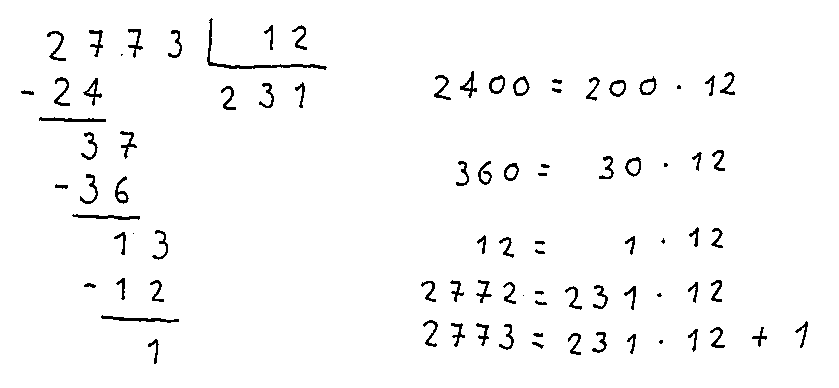
\includegraphics[width=7cm]{2020-1-C2/20201118_C2_div_com_resto_1.pdf}

\bsk

Com esta conta com polinômios:

% (find-fline "~/LATEX/2020-1-C2/20201118_C2_div_com_resto_2.pdf")
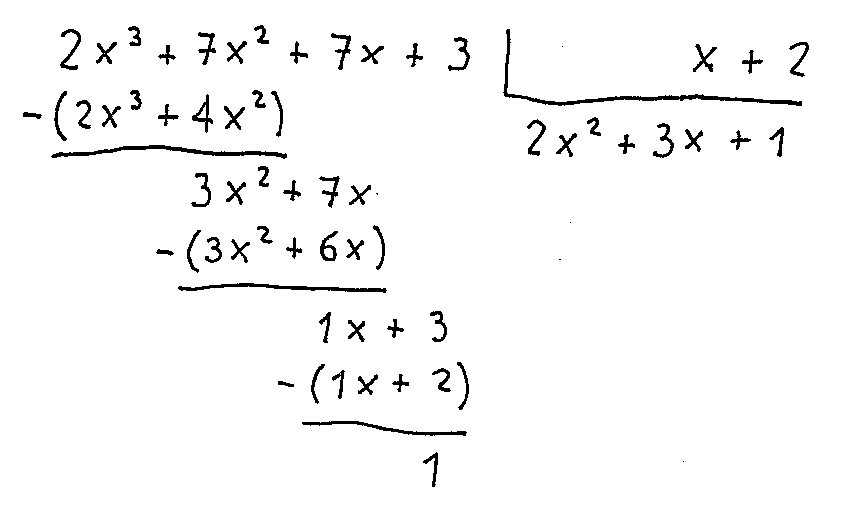
\includegraphics[width=5cm]{2020-1-C2/20201118_C2_div_com_resto_2.pdf}

% (find-fline "~/LATEX/2020-1-C2/20201118_C2_div_com_resto_3.pdf")
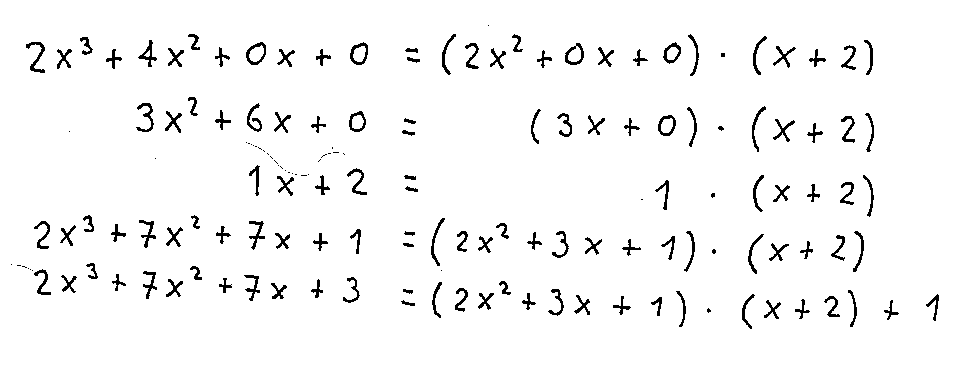
\includegraphics[width=7cm]{2020-1-C2/20201118_C2_div_com_resto_3.pdf}

}\anothercol{

{\bf Exercício 2}

Traduza a conta com polinômios da esquerda pra notação de caixinhas
daqui: \Ca{2xQ26}, \Ca{2yQ43}.

\bsk

{\bf Exercício 3}

Traduza a conta abaixo pra notação de caixinhas:
%
$$\begin{array}{l}
  \D \frac{2}{x+3} + \frac{4}{x-5} \\\\[-7pt]
  \D = \;\; \frac{2(x-5)}{(x+3)(x-5)} + \frac{(x+3)4}{(x+3)(x-5)} \\\\[-7pt]
  \D = \;\; \frac{2(x-5) + (x+3)4}{(x+3)(x-5)} \\\\[-7pt]
  \end{array}
$$

}}

\newpage

% «funcoes-racionais»  (to ".funcoes-racionais")
% (c2m231fpp 6 "funcoes-racionais")
% (c2m231fpa   "funcoes-racionais")

{\bf Funções racionais}

\scalebox{0.6}{\def\colwidth{10.5cm}\firstcol{

{\bf Exercício 4}

Entenda a definição de ``função racional própria'' daqui --
\Ca{Miranda240} -- e acrescente mais linhas nas contas do exercício 3
pra ``simplificar'' o resultado até ele virar uma ``função racional
própria''. Faça isso tanto na notação usual quanto na notação de
caixinhas.

\bsk

{\bf Exercício 5}

Entenda as contas do Exemplo 8.1 daqui -- \Ca{Miranda241} -- e
transforme a expressão abaixo numa função racional imprópria:
%
$$1000x^2 + 100x + 10 + \frac{2}{x+3} + \frac{4}{x-5}$$


\bsk

{\bf Exercício 6}

Isto aqui é verdade:
%
$$\frac{A}{x+3} + \frac{B}{x-5} = \frac{(A+B)x + (-5A+3B)}{x^2 - 2x - 15}
$$

mostre porquê ``aumentando o nível de detalhe'' -- transforme a
igualdade acima numa série de igualdades na qual cada passo seja bem
fácil de verificar.

}\anothercol{

{\bf Exercício 7}

Resolva:

\ssk

a) $(A+B)x + (-5A+3B) = 9x+11$

\ssk

b) $\D \frac{(A+B)x + (-5A+3B)}{x^2 - 2x - 15} = \frac{9x+11}{x^2 - 2x - 15}$

\ssk

c) $\D \frac{(A+B)x + (-5A+3B)}{x^2 - 2x - 15} = \frac{2x+7}{x^2 - 2x - 15}$

\ssk

d) $\D \frac{A}{x+3} + \frac{B}{x-5} = \frac{2x+7}{x^2 - 2x - 15}$

\ssk

e) $\D \intx{\frac{A}{x+3} + \frac{B}{x-5}}$

\ssk

f) $\D \intx{\frac{2x+7}{x^2 - 2x - 15}}$

\bsk
\bsk
\bsk

{\bf Exercício 8}

(Bem trabalhoso, pra casa!)

Mostre como organizar a solução do (7f) em

várias séries de igualdades fáceis de justificar,

como no slide 3. Você pode precisar de algumas

coisinhas em português, como na última página

do PDF de 2022.2: \Ca{2fT137}.





% (setq eepitch-preprocess-regexp "^%T ")
%
%T  (eepitch-maxima)
%T  (eepitch-kill)
%T  (eepitch-maxima)
%T f : A/(x+3) + B/(x-5);
%T ratsimp(f);

%T linsolve ([A+B, -5*A+3*B] - [2,7], [A, B]);
%T subst([A=2, B=7], [A+B, -5*A+3*B]);

% (find-es "maxima" "linsolve")


}}



\newpage

\standout{Aviso:} Todos os slides a partir daqui são antigos!

Assim que der eu vou fazer uma faxina neles

e deixar só o que ainda serve!!!




% «div-polis»  (to ".div-polis")
% (c2m222fpp 4 "div-polis")
% (c2m222fpa   "div-polis")
% (c2m202fpp 7 "div-polis")
% (c2m202fp    "div-polis")

\newpage

% «exercicio-1»  (to ".exercicio-1")
% (c2m222fpp 5 "exercicio-1")
% (c2m222fpa   "exercicio-1")

{\bf Exercício 1}

\sa{[RC]}{\CFname{RC}{}}
\sa {RC} {\ddx f(g(x)) = f'(g(x))g'(x)}
\sa{(RC)}{\left(\ga{RC}\right)}

Algumas consequências da regra da cadeia...
%
$$\ga{[RC]} \;=\; \ga{(RC)}$$

Obtenha os seguintes casos particulares da \ga{[RC]}:

\msk

a) $g(x) = 2x$

b) $g(x) = 2x+3$

c) $g(x) = x+3$

d) $g(x) = x+3$, $f(x)=\ln x$

e) $g(x) = -x$

f) $g(x) = -x$, $f(x) = \ln x$

g) $g(x) = -x+200$, $f(x) = \ln x$

\newpage

% «exercicio-2»  (to ".exercicio-2")
% (c2m222fpp 6 "exercicio-2")
% (c2m222fpa   "exercicio-2")
% (c2m201fracparcp 1 "title")
% (c2m201fracparc    "title")
% (c2m202fpp 2 "exercicio-1")
% (c2m202fp    "exercicio-1")


{\bf Exercício 2.}

\msk

a) $\D \intx{\frac{1}{3x}} = \ColorRed{?}$

\ssk

b) $\D \intx{\frac{1}{3x+4}} = \ColorRed{?}$

\ssk

c) $\D \intx{\frac{2}{3x+4}} = \ColorRed{?}$

\ssk

d) $\D \intx{\frac{a}{bx+c}} = \ColorRed{?}$


\newpage

% «derivadas-formais»  (to ".derivadas-formais")
% (c2m222fpp 7 "derivadas-formais")
% (c2m222fpa   "derivadas-formais")

{\bf Derivadas formais (de novo)}

Todas estas igualdades são verdadeiras,

mas se tentarmos formalizar elas com

todos os detalhes vamos ver que várias delas

falam de funções com domínios diferentes...
%
$$\begin{array}[t]{rcl}
  \ddx \ln x &=& \frac1x \\
  \ddx \ln (-x) &=& \frac1x \\
  \ddx \ln |x| &=& \frac1x \\
  \end{array}
  \qquad
  \begin{array}[t]{rcl}
  \intx{\frac1x} &=& \ln(x) \\
  \intx{\frac1x} &=& \ln(x) + C \\
  \intx{\frac1x} &=& \ln(-x) \\
  \intx{\frac1x} &=& \ln(-x) + C \\
  \intx{\frac1x} &=& \ln(|x|) \\
  \intx{\frac1x} &=& \ln(|x|) + C \\
  \intx{\frac1x} &=& 
    \begin{cases}
      \ln(-x) + C_1 & \text{quando $x<0$}, \\
      \ln(x) + C_2 & \text{quando $x>0$} \\
    \end{cases} \\
  \end{array}
$$




\newpage

%  _____                _   _               
% |_   _|__   __ _  ___| |_| |__   ___ _ __ 
%   | |/ _ \ / _` |/ _ \ __| '_ \ / _ \ '__|
%   | | (_) | (_| |  __/ |_| | | |  __/ |   
%   |_|\___/ \__, |\___|\__|_| |_|\___|_|   
%            |___/                          
%
% «together»  (to ".together")
% (c2m222fpp 8 "together")
% (c2m222fpa   "together")
% (c2m212fpp 3 "together")
% (c2m212fpa   "together")
% (c2m202fpp 3 "together")
% (c2m202fp    "together")
% (find-fline       "~/LATEX/2020-1-C2/20201112_C2_fracoes_parciais_2.pdf")
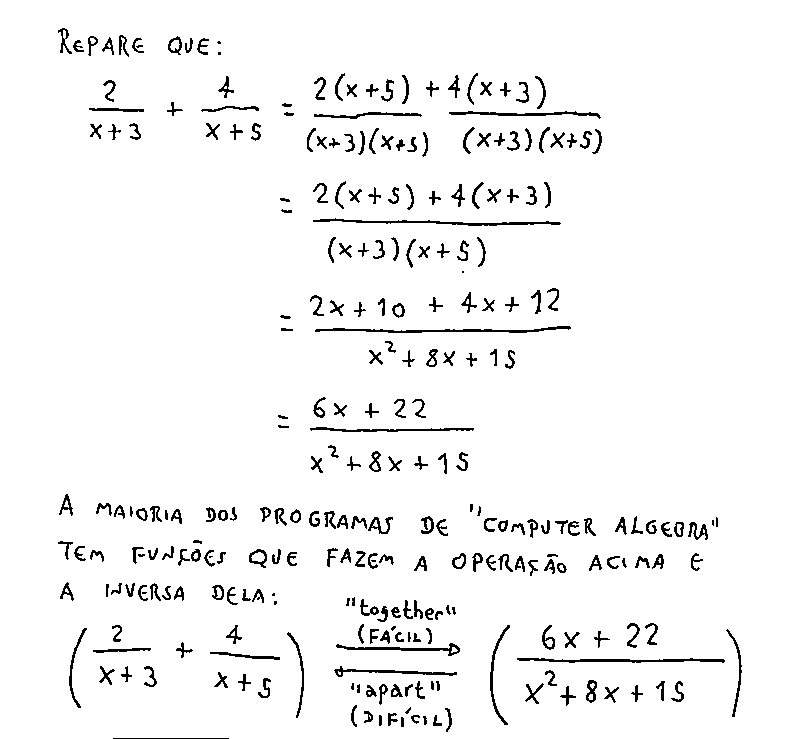
\includegraphics[height=8cm]{2020-1-C2/20201112_C2_fracoes_parciais_2.pdf}

% (find-es "sympy" "tut-apart")
% (find-es "sympy" "tut-together")
% (find-es "maxima" "partial-fractions")
% (setq eepitch-preprocess-regexp "^")
% (setq eepitch-preprocess-regexp "^%T ")
%
%T  (eepitch-isympy)
%T  (eepitch-kill)
%T  (eepitch-isympy)
%T f = 1/(x+1) + 1/(x-1)
%T f
%T g = together(f)
%T g
%T apart(g)
%T
%T  (eepitch-maxima)
%T  (eepitch-kill)
%T  (eepitch-maxima)
%T f : 2/(x+3) + 4/(x-5);
%T g : ratsimp(f);
%T ff : partfrac(g, x);

\newpage

% «exercicio-3»  (to ".exercicio-3")
% (c2m222fpp 9 "exercicio-3")
% (c2m222fpa   "exercicio-3")

{\bf Exercício 3.}

\msk

a) $\D \togetherp{\frac{1}{x+1} + \frac{1}{x-1}} = \ColorRed{?}$ 

\ssk

b) $\D \togetherp{\frac{A}{x-a} + \frac{B}{x-b}} = \ColorRed{?}$ 

\ssk

c) $\D \togetherp{\frac{A}{x-a} + \frac{B}{x-b} + \frac{C}{x-c}} = \ColorRed{?}$ 

%        (find-fline "~/LATEX/2020-1-C2/20201112_C2_fracoes_parciais_3.pdf")
%\includegraphics[height=7cm]{2020-1-C2/20201112_C2_fracoes_parciais_3.pdf}

\newpage

% «exercicio-4»  (to ".exercicio-4")
% (c2m222fpp 10 "exercicio-4")
% (c2m222fpa    "exercicio-4")
% (c2m212fpp 5 "exercicio-3")
% (c2m212fpa   "exercicio-3")

{\bf Exercício 4.}

% (find-fline "~/LATEX/2020-1-C2/20201112_C2_fracoes_parciais_4.pdf")
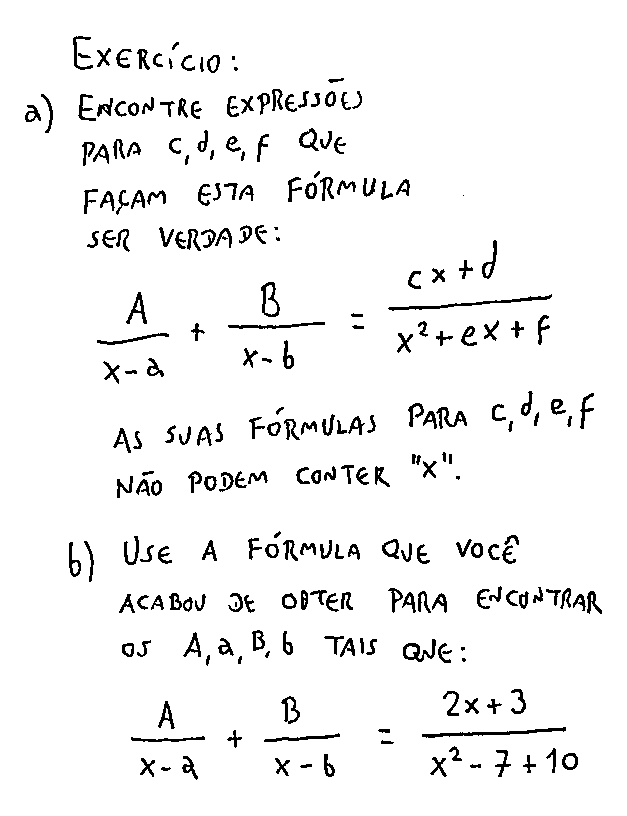
\includegraphics[height=7cm]{2020-1-C2/20201112_C2_fracoes_parciais_4.pdf}

\newpage

% «exercicio-4a»  (to ".exercicio-4a")
% (c2m222fpp 11 "exercicio-4a")
% (c2m222fpa    "exercicio-4a")
% (c2m212fpp 6 "exercicio-3-maxima")
% (c2m212fpa   "exercicio-3-maxima")
% (find-es "maxima" "partial-fractions")

{\bf Exercício 4: uma solução pro item (a)}

% (setq eepitch-preprocess-regexp "^")
% (setq eepitch-preprocess-regexp "^%T ")
%
%T  (eepitch-maxima)
%T  (eepitch-kill)
%T  (eepitch-maxima)
%T f1 : A/(x-a) + B/(x-b);
%T f2 : ratsimp(f1);
%T (f1 = f2);
%T f3 : (c*x+d) / (x^2+e*x+f); 
%T fs : [e=-a-b, f=a*b, c=A+B, d=-A*b-a*B];
%T f4 : subst(fs, f3);
%T f2 - f4;
%T 
%T g1 : (2*x + 3) / (x^2 - 7*x + 10)$
%T g2 : partfrac(g1, x)$
%T (g1 = g2);
%T g2;
%T f1;
%T gs : [b=5, B=13/3, a=2, A=-7/3];
%T subst(gs, f1);
%T ratsimp(subst(gs, f1) - g1);

\sa{f1}{\frac{A}{x-a} + \frac{B}{x-b}}
\sa{f1.5}{\frac{A(x-b)}{(x-a)(x-b)} + \frac{B(x-a)}{(x-a)(x-b)}}
\sa{f1.6}{\frac{A(x-b) +                    B(x-a)}{(x-a)(x-b)}}
\sa{f2}{\frac {(A+B)x + (-Ab-Ba)} {x^2 + (-a-b)x + ab}}
\sa{f3}{\frac {cx+d} {x^2+ex+f}}
\sa{g1}{\frac {2x+3} {x^2-7x+10}}
\sa{g2}{\frac {2x+3} {(x-2)(x-5)}}
\sa{g3}{\frac {A(x-2)} {(x-2)(x-5)} + \frac {B(x-5)} {(x-2)(x-5)}}

\msk

a) $\scalebox{1.0}{$
    \begin{array}[t]{rcl}
      \ga{f1} &=& \ga{f3}   \\[7pt]
      \ga{f1} &=& \ga{f1.5} \\[6pt]
              &=& \ga{f1.6} \\[6pt]
              &=& \ga{f2}   \\[7pt]
            c &=& A+B    \\
            d &=& -Ab-Ba \\
            e &=& -a-b   \\
            f &=& ab     \\[15pt]
    \end{array}
    $}
   $

\newpage

% «exercicio-4a-2»  (to ".exercicio-4a-2")
% (c2m222fpp 12 "exercicio-4a-2")
% (c2m222fpa    "exercicio-4a-2")

{\bf Exercício 4: uma solução pro item (a), cont...}

\scalebox{0.6}{\def\colwidth{9cm}\firstcol{

Dá pra gente reescrever isso usando o `$[:=]$':
%
$$\begin{array}{l}
  \left( \ga{f1} \;\;=\;\; \ga{f3} \right)
    \bsm{ c:=A+B \\ d:=-Ab-Ba \\ e:=-a-b \\ f:=ab} \\[15pt]
  = \left( \ga{f1} \;\;=\;\; \ga{f2} \right),
 \end{array}
$$

e sabemos que esta igualdade é verdade:
%
$$\ga{f1} \;\;=\;\; \ga{f2}$$

então isto aqui
%
$$\begin{array}{rcl}
    c &=& A+B \\
    d &=& -Ab-Ba \\
    e &=& -a-b \\
    f &=& ab \\
  \end{array}
$$

é \ColorRed{uma} solução para a equação
%
$$\ga{f1} \;\;=\;\; \ga{f3} \;\; ...$$

mas não sabemos se é a \ColorRed{única} solução!

}\anothercol{

Sempre dá pra escrever soluções de equações

usando o `$[:=]$'. Por exemplo, as duas soluções

da equação
%
$$ (x-2)(x-5) = 0:$$

São:
%
$$\begin{array}{l}
    \left( (x-2)(x-5)=0 \right) [x:=2] \; = \\
    \left( (2-2)(2-5)=0 \right)             \\
    \left( (x-2)(x-5)=0 \right) [x:=5] \; = \\
    \left( (5-2)(5-5)=0 \right)             \\
  \end{array}
$$

\ColorRed{Nenhum} livro ``\ColorRed{básico}'' define

``solução de uma equação'' desse jeito ---

como ``a substituição que transforma a

equação numa igualdade verdadeira'' ---

mas eu acho isso um bom modo de

entender o que são ``equações'' e

``soluções''...

\msk

Ah, note que eu não fiquei repetindo a

condição ``as suas fórmulas para $c,d,e,f$

não podem conter `$x$'\,'' o tempo todo...

eu deixei isso implícito. \quad \smile


}}


\newpage

% «exercicio-4b»  (to ".exercicio-4b")
% (c2m222fpp 13 "exercicio-4b")
% (c2m222fpa    "exercicio-4b")

{\bf Exercício 4: uma solução pro item (b)}


\scalebox{1.0}{\def\colwidth{9cm}\firstcol{

Temos duas soluções para
%
$$(x-a)(x-b) = x^2-7x+10:$$

uma é $a=2$ e $b=5$, e a outra é $a=5$ e $b=2$.

Lembre que Cálculo 2 é sobre \ColorRed{chutar} e \ColorRed{testar}.

A gente pode chutar que $a=5$, $b=2$, e que

$c,d,e,f$ são os que a gente obtém pelo

item (a), e aí ver se isso nos leva a uma

solução...

\msk

(Obs: isso funciona!!!) 

}\anothercol{
}}





\newpage

% «exercicio-4c»  (to ".exercicio-4c")
% (c2m222fpp 14 "exercicio-4c")
% (c2m222fpa    "exercicio-4c")
% (c2m212fpp 9 "exercicio-3c")
% (c2m212fpa   "exercicio-3c")
% (find-books "__analysis/__analysis.el" "miranda")
% (find-dmirandacalcpage 246 "8.1.2 Fatores quadráticos")
% (find-dmirandacalcpage 251 "Exercícios")

{\bf Exercício 4: item (c)}

Seja [PFP] esta igualdade aqui -- o

``princípio por trás das frações parciais'':
%
$$\text{[PFP]} \;\;=\;\;
  \left(\ga{f1} \;\;=\;\; \ga{f1.6}
  \right)
$$

\msk

c) Resolva o exercício 8.7.2 do livro do Miranda --

\ssk

{\scriptsize

\url{http://hostel.ufabc.edu.br/~daniel.miranda/calculo/calculo.pdf#page=251}

}

\ssk

\def\rq{\ColorRed{?}}

e depois mostre qual é a substituição da forma
%
$$\text{[PFP]} \bsm{a:=\rq \\ b:=\rq \\ A:=\rq \\ B:=\rq}
$$

que ``está por trás'' da sua solução.



\newpage

% «exercicio-5»  (to ".exercicio-5")
% (c2m222fpp 15 "exercicio-5")
% (c2m222fpa    "exercicio-5")
% (c2m201fracparcp 8 "exercicio-4")
% (c2m201fracparc    "exercicio-4")

{\bf Exercício 5.}

\ssk

Use estas idéias para integrar:

$$\intx{\frac{2x^3 + 7x^2 + 7x + 3}{x+2}} \;\; = \;\; ?$$



\newpage

% «exercicio-6»  (to ".exercicio-6")
% (c2m222fpp 16 "exercicio-6")
% (c2m222fpa    "exercicio-6")

{\bf Exercício 6.}

\ssk

O que acontece nos casos em que ``teria vai um''?

\ssk

a) Tente fazer a divisão com resto de $x^3$ por $x+2$.

Mais precisamente, encontre um polinômios $R(x)$ e $Q(x)$ tais que

$(x^3) = Q(x) · (x+2) + R(x)$ e $R(x)$ é no máximo de grau 1.

Teste a sua resposta!

\ssk

b) Calcule $\intx{\frac{x^3}{x+2}}$ pelo método acima.

Teste a sua resposta derivando a sua antiderivada para $\frac{x^3}{x+2}$.

\ssk

c) Calcule $\intx{\frac{x^3}{x+2}}$ fazendo a substituição $u=x+2$.

Você deve obter o mesmo resultado que na (b).

\bsk

d) Calcule $\intx{\frac{x^2}{(x+1)(x-1)}}$ por frações parciais.


\newpage

{\bf Dica importante}

\ssk

Lembre que uns dos meus slogans é

``eu só vou corrigir os sinais de igual''...

No slide ?? a igualdade mais importante é a da última linha.

Nós vamos usá-la assim, pra transformar a integral original

em algo fácil de integrar:

\msk

% (find-fline "~/LATEX/2020-1-C2/20201119_C2_div_com_resto_4.pdf")
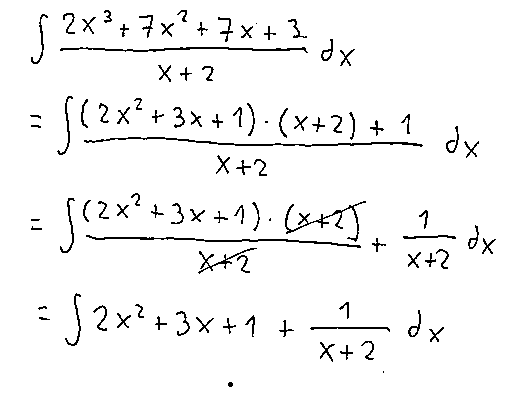
\includegraphics[height=4cm]{2020-1-C2/20201119_C2_div_com_resto_4.pdf}


\newpage

% «P1-2020.1»  (to ".P1-2020.1")
% (c2m202fpp 11 "P1-2020.1")
% (c2m202fp     "P1-2020.1")

{\bf Uma questão da P1 de 2020.1}

A questão 3 da P1 de 2020.1,

\ssk

% (c2m201p1p 5 "questao-3")
% (c2m201p1    "questao-3")
% (c2m201p1p 9 "gabarito-3a")
% (c2m201p1a   "gabarito-3a")
%    http://angg.twu.net/LATEX/2020-1-C2-P1.pdf
\url{http://angg.twu.net/LATEX/2020-1-C2-P1.pdf}

\ssk

era de frações parciais, e eu pus nesse PDF um gabarito

parcial dela, que não inclui nem as contas da divisão de

polinômios nem a verificação de que a nossa integral

está certa. Faça a questão, incluindo a parte que

não está no gabarito.



\GenericWarning{Success:}{Success!!!}  % Used by `M-x cv'

\end{document}


% Local Variables:
% coding: utf-8-unix
% ee-tla: "c2fp"
% ee-tla: "c2m231fp"
% End:
